\section{Aerospace State Estimation}

\subsection{Sensor Measurement} \label{s:measurements}

During the standard estimation procedure, it is assumed that
measurements are made that relate to the state or the state is
directly measured. If the state is directly measured like star trackers no special formulation need to
made. However, other sensors such as Sun sensors, magnetometers and
horizon sensors measure a vector in 3-D space. In general a
measurement $\bar{y}_k$ can be expressed by the nonlinear equation
shown below where $\vec{x}$ is the state vector. 
\begin{equation}
  \bar{y}_k = \vec{h}(\vec{x}_k) + \vec{\nu}_k
\end{equation}
The vector $\vec{\nu}_k$ is noise associated with the sensor
\cite{Munoz,cassidis}. If the system is linearized about some
equilibrium point the measurement equation can be written as
\begin{equation}
  \bar{y}_k = {\bf h}_k\vec{x}_k + \vec{\nu}_k
\end{equation}
where ${\bf h}_k = \partial \vec{h}/\partial \vec{x}$. 
It's easy to see here that in the case of the star tracker the matrix
${\bf h}_k$ is just the identity matrix. The noise vector
$\vec{\nu}_k$ is assumed to be gaussian white noise while the
covariance $cov()$ is given by the equation below using the
expectation operator ${\bf E}()$.
\begin{equation}
  cov(\vec{\nu}_k) = {\bf E}(\vec{\nu}_k\vec{\nu}_k^T) = {\bf R}_k
\end{equation}
If a measurement is made by a
Sun sensor or similar where a vector in 3-D space can be compared to a
known inertial reference vector the measurement update can be given as 
\begin{equation}
  {\bar{r}^B}_k = {\bf T}_{BI}(\vec{q}_k){\vec{r}^I}_k + \vec{\nu}_k
\end{equation}
where ${\bar{r}^B}_k$ is a measurement in the body reference frame at
time $t_k$. The angular velocity measurement in particular can be denoted as
$\bar{\omega}_k$. Measurements are typically polluted with bias and
white noise. For example, the angular velocity measurement can be
given as
\begin{equation}
  \bar{\omega} = \vec{\omega} + \vec{b} + \vec{\eta}_g
\end{equation}
where $\vec{b}$ is a bias that has dynamics given by
$\dot{\vec{b}}=\vec{\eta}_b$. The vectors $\vec{\eta}_g$ and
$\vec{\eta}_b$ are standard Gaussian white noise vectors. Typically
white noise can be filtered out using lowpass filters, complimentary
filters or even Kalman Filters while bias can just be
substracted. Thus, the estimate for the angular velocity can be
written as
\begin{equation}
  \tilde{\omega} = \bar{\omega}-\tilde{b}
\end{equation}
where $\tilde{b}$ is the estimate of the bias.

\subsection{Linear Least Squares}

In order to understand the nature of a Kalman filter, the linear least
squares solution is shown below. Assume for the moment that $M$
independent measurements are made such that $\bar{Y} = [\bar{y}_1,...,\bar{y}_M]^T$.
\begin{equation}
  \bar{Y} = {\bf H}\vec{x} + \vec{V}
\end{equation}
In this case ${\bf H} = [{\bf h}_1,...,{\bf h}_M]^T$ and $\vec{V} = [\nu_1,...,\nu_M]^T$. 
The vector $\vec{V}$ is a vector of error values between your
measurements and the actual truth signals $Y = {\bf H}\vec{x}$. Absent
of all measurement and model noise there 
would be a unique solution to this problem to solve for the vector
$\vec{x}$. The matrices $\bar{Y}$ and {\bf H} are
known and are the measurements and the output equation relating the
measurements to the state values in $\vec{x}$ respectively. Because of
measurement and model noise, a unique solution is not possible. That
is, the problem is overconstrained since typically the number of measurements is larger
than the number of unknowns. Take the linear example as shown in the
figure below.
\begin{figure}[H]
  \begin{center}
  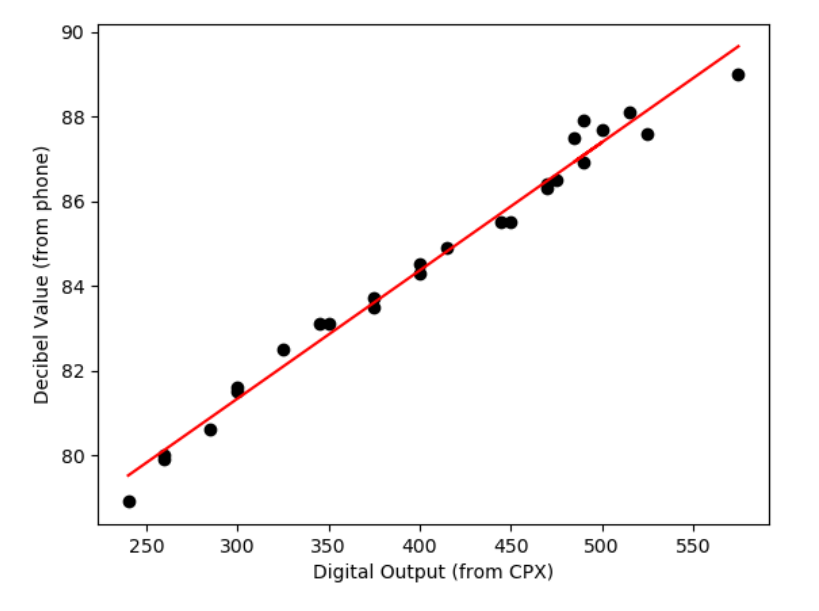
\includegraphics[height=80mm, width=100mm]{Figures/Linear_Regression.png}
  \end{center}
  \caption{Linear Regression Example}\label{f:linear_regression}
\end{figure}
In this case the ordinate axis is the output $Y$ and the abscissa is
the independent variable that characterizes the matrix ${\bf H}$. The
black dots then are the measurements $\bar{Y}$ while the trend line is
the estimate $\tilde{Y} = {\bf H}\tilde{x}$. In this case the residuals
$\hat{Y} = \tilde{Y}-\bar{Y}$ is the distance between the trend line
in red and the black dots (the measurements). For this linear example,
the unknowns would be the slope and intercept. It is clear here that
there exists no linear solution $\vec{x}$ that goes through all black
data points. Thus, the equation below can be constructed.
\begin{equation}
  \bar{Y} = {\bf H}\tilde{x} + \hat{Y}
\end{equation}
This implies that the trendline $\tilde{Y}$ would go through all data
points if $\hat{Y}$ were zero. Thus the solution to this problem was
originally found by Gauss \cite{stigler1981} and involved minimizing
the residuals between $\bar{Y}$ and $\tilde{Y}$ (the estimated Y
values). To do this, a cost function is generated such that
\begin{equation}
  J = \frac{1}{2}\hat{Y}^T \hat{Y}
\end{equation}
Substituting in the equation $\hat{Y} = \bar{Y} - {\bf H}\tilde{x}$
and minimizing the cost function $\partial J/\partial \tilde{x} = 0$
results in the solution below.
\begin{equation}
  \tilde{x} = ({\bf H}^T{\bf H})^{-1}{\bf H}^T\bar{Y}
\end{equation}
Note that the equation above only works if the number of measurements $M$
is greater than or equal to the number of unknowns $N$. If not, the
solution will always be rank deficient and no solution will be
found. This is called an under constrained problem. In this there are
an infinite number of solutions that satisfy $\bar{Y} = {\bf
  H}\vec{x}$ even in the presence of modeling errors. In order
to get around this issue Lagrange's method of 
optimization is used \cite{lagrange}. For problems like this the
residuals between the estimate $\tilde{Y}$ and the measured signals
$\bar{Y}$ can be easily made to be zero. Thus minimizing the residuals
is trivial since the solution will still be an infinite number of
solutions. Therefore a constraint can be placed where
$\bar{Y}=\tilde{Y}={\bf H}\tilde{x}$. In order to find a unique
solution then the requirement is placed to minimize the estimate
$\tilde{x}$. In this case, the cost function
to be minimized is given by Lagrange's extension to optimization as
shown below
\begin{equation}
L = \frac{1}{2}\tilde{x}^T\tilde{x} + \lambda^T(\bar{Y}-{\bf H}\tilde{x})
\end{equation}
The cost function above utilizes the method of Lagrange multipliers in
order to satisfy the constraint that the solution must pass through
all measurements again only if the number of measurements $M$ is less than
the number of unknowns $N$. In the equation above the vector
$\tilde{x}$ must be solved and so must the Lagrange multipliers
$\lambda$. The solution to the problem above requires
$\partial L / \partial \tilde{x} = 0$ and $\partial L / \partial \lambda = 0$. Carrying out the partial derivatives and solving for the estimate
yields the following equations. 
\begin{equation}
  \tilde{x} = {\bf H}^T({\bf H}{\bf H}^T)^{-1}\bar{Y}
\end{equation}
Note, it is standard practice in state estimation to have at least as
many measurements as unknowns. In this case $M=N$ and Gauss' solution
is sufficient. 

\subsection{Weighted Least Squares}

The weighted least squares solution is found by setting the cost
function equal to $J = \frac{1}{2}\hat{Y}^T{\bf W}\hat{Y}$
where {\bf W} is a positive definite and symmetric weighting matrix. The solution then is
shown below.
\begin{equation}\label{e:weights}
  \tilde{x} = ({\bf H}^T{\bf W}{\bf H})^{-1}{\bf H}^T{\bf W}\bar{Y}
\end{equation}
In the standard Kalman Filter approach, the weighting matrix is given
by the inverse covariance of the error ${\bf r} = {\bf
  E}[\vec{v}\vec{v}^T]$. Placing this into a matrix yield ${\bf W} =
{\bf R}^{-1}$ where ${\bf R} = diag([{\bf r}_1,...{\bf r}_M])$.  
The weighted least squares solution then reduces to
\begin{equation}
  \tilde{x} = ({\bf H}^T{\bf R}^{-1}{\bf H})^{-1}{\bf H}^T{\bf R}^{-1}\bar{Y}
\end{equation}

\subsection{A Priori Knowledge of the State Vector}

If a priori knowledge is obtained via other means or in the case of
the standard Kalman Filter from integration of the state, it is
possible to obtain an updated estimate of the state based on the
previous state estimate and the new sensor measurements. First, the a
priori estimate $\tilde{x}^{-}$ is written as 
\begin{equation}
  \tilde{x}^{-} = \vec{x} +  \vec{w}
\end{equation}
where $\vec{w}$ is model noise associated with the error in the
state estimate. The covariance of this noise is also denoted as a
matrix and defined below.
\begin{equation}
  cov(\vec{w}) = {\bf E}(\vec{w}\vec{w}^T) = {\bf q}
\end{equation}
In this case it is desired for the updated measurement to be some
linear combination of the a priori equation and the measurements such
that
\begin{equation}
  \tilde{x} = {\bf \Lambda}\bar{Y} + {\bf \Gamma}\tilde{x}^{-}
\end{equation}
The matrices ${\bf \Lambda}$ and ${\bf \Gamma}$ have an added constraint
which can be shown by assuming the a priori measurement is perfect
$\tilde{x}^- = \vec{x}$ and the measurements $\bar{Y} = Y = {\bf
  H}\vec{x}$. In this case, we must have the updated estimate equal
the truth signal. $\tilde{x} = \vec{x}$. Rearranging the equation above yields
\begin{equation}
  \vec{x} = {\bf \Lambda}{\bf H}\vec{x} + {\bf \Gamma}\vec{x}
\end{equation}
which means that $({\bf \Lambda}{\bf H} + {\bf \Gamma}) = {\bf I}$
Again using the method of lagrange multipliers the cost function to be
minimized is given as
\begin{equation}
  L = {\bf E}[\frac{1}{2}\hat{x}^T\hat{x} + \lambda^T({\bf I} - {\bf
    \Lambda}{\bf H} - {\bf \Gamma})]
\end{equation}
where $\hat{x} = \tilde{x} - \vec{x}$ and again {\bf E} is the
expectation operator. Remembering that {\bf q} is
the covariance of the model noise and {\bf r} is the covariance of the
measurement noise, the solution to the minimization problem is given
by the equation below. 
\begin{equation}
  \tilde{x} = ({\bf H}^T{\bf R}^{-1}{\bf H}+{\bf q}^{-1})^{-1}({\bf
    H}^T{\bf R}^{-1}\bar{Y}+{\bf q}^{-1}\tilde{x}^{-})
\end{equation}
Note that this solution assumes that ${\bf E}(\vec{w}\vec{v}^T) = 0$. Measurement and model noise are uncorrelated.

\subsection{Complimentary Filter}

Looking at the equation for the A priori knowledge it is possible to
formulate the complimentary filter. First, the measurements are
assumed to be identical to the state vector such that ${\bf h}_k = {\bf
  I}$. From here a few extremes are shown below. First, assume that the measurement error is very low such
that the $cov(\vec{\nu})<<1$ while the model noise $\vec{w}$ is very
large approaching infinity. In this case, ${\bf q}^{-1} =0$. Substituting this into the weighted apriori equation yields
\begin{equation}
  \tilde{x} = average(\bar{Y})
\end{equation}
which essentially states that the estimate completely believes the
sensor measurement. If instead we assume that the model noise is
perfect such that $cov(\vec{w})<<1$ and the sensor noise is
approaching infinity, then ${\bf R}^{-1}=0$. This yields the following equation.
\begin{equation}
  \tilde{x} = \tilde{x}^{-}
\end{equation}
Thus it can be seen that there is a sliding bar between believing the
apriori estimate or the sensor measurement. As such it is possible to
develop a much simpler filter. First a constraint is placed on {\bf q}
and {\bf R} such that
\begin{equation}
  ({\bf H}^T{\bf R}^{-1}{\bf H}+{\bf q}^{-1}) = {\bf I}
\end{equation}
This causes the update law to reduce to the following
\begin{equation}
  \tilde{x} = {\bf H}^T{\bf R}^{-1}\bar{Y}+{\bf q}^{-1}\tilde{x}^{-}
\end{equation}
If only one measurement is investigated the equation collapses to the
following.
\begin{equation}
  \tilde{x} = {\bf r}^{-1}\bar{y}+{\bf q}^{-1}\tilde{x}^{-}
\end{equation}
The constraint also collapses to
\begin{equation}
  {\bf r}^{-1}+{\bf q}^{-1} = {\bf 1}
\end{equation}
If ${\bf q}^{-1} = {\bf s}$ and ${\bf r}^{-1}={\bf 1}-{\bf s}$ the
update law simplifies to
\begin{equation}
  \tilde{x} = ({\bf 1}-{\bf s})\bar{y}+{\bf s}\tilde{x}^{-}
\end{equation}
Here it is clear that if ${\bf s} = {\bf 1}$ the new estimate will be
equal to the old estimate meaning that the sensor noise is approaching
infinite. If ${\bf s} = 0$ it means that the new estimate is equal to
the sensor measurement meaning the model noise is approaching
infinity. This is a simple crude first order filter that can be used
when only a simple understanding of covariance is known.

\subsection{Sequential Linear Estimator}

In the above two scenarios, it is assumed that all measurements from 1
to $M$ are known at the same time instant $t$ and thus the least squares estimate can be done ``all
at once". For discrete time sensors on board a spacecraft this is
not possible. For example, if we take the weighted least squares
solution assuming we have a {\it 0th} batch of measurements, the
estimate of $\tilde{x}$ would be
\begin{equation}
  \tilde{x}_0 = ({\bf h}_0^T{\bf w}_0{\bf h}_0)^{-1}{\bf h}_0^T{\bf
    w}_0\bar{y}_0
\end{equation}
If we then waited $\Delta t$ seconds for a new set of measurements we
would have to obtain a new estimate of $\tilde{x}$ which could be done
using the equation below
\begin{equation}
  \tilde{x}_1 = ({\bf h}_1^T{\bf w}_1{\bf h}_1)^{-1}{\bf h}_1^T{\bf
    w}_1\bar{y}_1
\end{equation}
This solution however would only take into account the new
measurements. Thus, if larger matrices were constructed like
${\bf H} = [{\bf h}_0,{\bf h}_1]$ the solution for $\tilde{x}$ becomes
the same as it was in Equation \ref{e:weights}. This process would be
tedious if these matrices were computed over and over again. This is
because the matrices would continue to grow larger and larger over
time and eventually overflow the memory management system on the
computer. Thus, a method for updating the state vector every time
a new measurement is obtained must be derived. To do this the two
equations are substituted into equation \ref{e:weights}. Then a
covariance matrix is used such that ${\bf p} = ({\bf h}^T{\bf w}{\bf h})^{-1}$ 
which never grows in size. Using that simplification and making use of
a estimation gain matrix ${\bf k}$, the estimation algorithm is as follows:
\begin{enumerate}[itemsep=-5pt]
    \item The first measurement is obtained $\bar{y}_0$
    \item Compute the matrix ${\bf p_0} = ({\bf h}_0^T{\bf w_0}{\bf h}_0)^{-1}$
    \item Obtain the estimate for $\tilde{x}_0 = {\bf p_0}{\bf
      h}_0^T{\bf w_0}\bar{y}_0$ (Notice that if you use the equation
      above this is the same solution as the weighted least squares estimate)
    \item Every time a new measurement, $\bar{y}_k$, is obtained use the recursive least squares update law shown in the equation below.  
\end{enumerate}
\begin{equation}
  \begin{matrix}
    {\bf k}_{k+1} = {\bf p}_{k}{\bf h}_{k+1}^T[{\bf h}_{k+1}{\bf p}_k{\bf h}_{k+1}^T+{\bf w}_k^{-1}]^{-1}\\
    {\bf p}_{k+1} = [{\bf 1} - {\bf k}_{k+1}{\bf h}_{k+1}]{\bf p}_k\\
    \tilde{x}_{k+1} = \tilde{x}_k + {\bf k}_{k+1}(\bar{y}_{k+1} - {\bf h}_{k+1}\tilde{x}_k) \\
  \end{matrix}
\end{equation}
In the special case where the weighting matrix
${\bf w}_k$ is equal to a constant ${\bf w}$ and the state vector is
directly measured such that ${\bf h}_k$ is also identity, the 
sequential linear estimator gives the following simplified steps.
\begin{enumerate}[itemsep=-5pt]
    \item The first measurement is obtained $\bar{y}_0$
    \item Compute ${\bf p}_0 = {\bf w}^{-1}$
    \item Obtain the estimate for $\tilde{x}_0 = \bar{y}_0$ (this is a fault of ${\bf h}_k$ being identity) 
    \item Every time a new measurement, $\bar{y}_k$, is obtained use the recursive least squares update law shown in the equation below.  
\end{enumerate}
\begin{equation}
  \begin{matrix}
    {\bf k}_{k+1} = {\bf p}_k[{\bf p}_k + {\bf w}^{-1}]^{-1}\\ 
    {\bf p}_{k+1} = [{\bf 1} - {\bf k}_{k+1}]{\bf p}_k\\
    \tilde{x}_{k+1} = \tilde{x}_k + {\bf k}_{k+1}(\bar{y}_{k+1} - \tilde{x}_k) \\
  \end{matrix}
\end{equation}

\subsection{The Continuous Time Complimentary Filter}

In the above section a discrete sequential least squares update law
was formulated. In that derivation it is assumed that the state
estimate is held constant in between state measurements. It is
possible however to integrate a model of the state dynamics and use
that estimate in between state measurements. The is the start of a
Kalman Filter. To formulate the Continuous Time Complimentary Filter
the dynamics of the system are written such that
\begin{equation}
  \begin{matrix}
    \dot{\vec{x}} = {\bf f}\vec{x} + {\bf g}u +{\bf m}\vec{w} \\
    \vec{y} = {\bf h}\vec{x}
  \end{matrix}
\end{equation}
where the initial conditions are $\vec{x}_0$ and $\vec{w}$ is a
modeling noise term where ${\bf E}[\vec{w}\vec{w}^T]={\bf q}$ just as
was defined in the a priori estimation section. The model dynamics are
set up such that 
\begin{equation}
  \begin{matrix}
    \dot{\tilde{x}} = \tilde{{\bf f}}\tilde{x} + \tilde{{\bf g}}u + \vec{\gamma}\\
    \tilde{y} = {\bf h}\tilde{x} \\
    \bar{y} = {\bf h}\vec{x} + \vec{v}
  \end{matrix}
\end{equation}
where again $\bar{y}$ is the state measurement and $\vec{v}$ is noise
associated with the sensor where {\bf E}$[\vec{v}\vec{v}^T]=${\bf
  r}. The term $\vec{\gamma}$ is added as a psuedo control which can
be whatever we want. The idea is for $u$ to be the control input to
drive $\vec{x} \rightarrow \vec{x}_c$ while the psuedo control is for
the observer dynamics to drive $\tilde{y} \rightarrow \bar{y}$. The
model dynamics are going to deviate in between sensor measurements so
if the observer dynamics are designed properly the estimate can
converge to the measurement. Of course, this means your estimate is
only as good as your measurement noise but it is a start. To design
the psuedo control law, measurement feedback is used in the same form
as standard unity feedback control laws such that $\vec{\gamma} =
{bf k}\hat{y}$ where $\hat{y}$ is the difference between the estimate and
the measurement. The closed loop dynamics can then be written as
\begin{equation}
  \dot{\tilde{x}} = (\tilde{{\bf f}}-{\bf k}{\bf h})\tilde{x} + \tilde{{\bf g}}u
  + {\bf k}\bar{y}
\end{equation}
Looking at this equation it's hard to see the effect of the
observer. Thus the error dynamics must be investigated where
$\hat{x}=\tilde{x}-\vec{x}$. For the simple case it is assumed that
${\bf f}=\tilde{{\bf f}}$ and ${\bf g}=\tilde{{\bf g}}$. The closed
loop error dynamics can then be written as
\begin{equation}
  \dot{\hat{x}} = ({\bf f} - {\bf k}{\bf h})\hat{x} + {\bf k}\vec{v}
\end{equation}
in this case the solution to this equation is
\begin{equation}
  \hat{x}(t) = \hat{x}_0e^{({\bf f} - {\bf k}{\bf h})t} + \vec{\eta}
\end{equation}
where the term $\vec{\eta}$ is a function of the noise term ${\bf
  k}\vec{v}$. In this case, if {\bf k} is chosen to be large, the
error dynamics will be very fast but the noise term will be very
large. If {\bf k} is chosen to be very small the error dynamics will
be slow but the error term will not be a prevalent. The issue with
this filter of course comes with how to tune the gain matrix {\bf k}
which is what the Kalman filter seeks to address.
   
\subsection{The Continuous Discrete Kalman Filter}

In the case of the continuous discrete Kalman Filter, the model
dynamics are integrated just as in the complimentary filter. The only
difference is instead of using a continuous observer the state
estimate is updated every time a new measurement is obtained much like
the sequential least squares technique. First, let's write the model
dynamics as before without the observer and the measurement equations
are written such that the measurement is taken at timestep $t_k$ and
thereafter every $\Delta t$. 
\begin{equation}\label{e:model_dynamics}
  \begin{matrix}
    \dot{\tilde{x}} = \tilde{{\bf f}}\tilde{x} + \tilde{{\bf g}}u \\
    \tilde{y} = {\bf h}\tilde{x} \\
    \bar{y}_k = {\bf h_k}\vec{x}(t_k) + \vec{v}_k
  \end{matrix}
\end{equation}
The update equation is written using the continuous observer dynamics
used for the complimentary filter only in this case the update is
discrete.
\begin{equation}\label{e:state_update}
  \tilde{x}_k^+ = \tilde{x}_k^- + {\bf k}_k(\bar{y}_k-{\bf
    h_k}\tilde{x}_k^-)
\end{equation}
In this case $\tilde{x}_k^+$ is the estimated state after the update
while $\tilde{x}_k^-$ is the estimate before the update. The equation
for the covariance update and the Kalman Gain matrix are identical in
that the derivation is formulated just as it was before. The equations
are shown below again only $+$ and $-$ is used to denote the matrices
before and after update.
\begin{equation}\label{e:kalman_gain}
  \begin{matrix}
  {\bf k}_{k} = {\bf p}_{k}{\bf h}_{k}^T[{\bf h}_{k}{\bf p}_k^-{\bf h}_{k}^T+{\bf r}]^{-1}\\
  {\bf p}_{k}^+ = [{\bf 1} - {\bf k}_{k}{\bf h}_{k}]{\bf p}_k^-
  \end{matrix}
\end{equation}
In the sequential linear estimator however, the covariance matrix was
set using a weighted least squares approach. In this case the
covariance matrix is set such that ${\bf p} = {\bf
  E}[\hat{x}\hat{x}^T]$. Taking a derivative of this equation and
substituting in the closed loop error dynamics yields the covariance
propagation equation shown below.
\begin{equation}\label{e:covariance_dynamics}
  \dot{{\bf p}} = \tilde{{\bf f}}{\bf p} + {\bf p}\tilde{{\bf f}}^T +
      {\bf m}{\bf q}{\bf m}^T
\end{equation}
The final Continuous Discrete Kalman Filter then goes like this.
\begin{enumerate}
  \item Integrate the model dynamics in Equation
    \ref{e:model_dynamics} and the covariance dynamics in equation
    \ref{e:covariance_dynamics}
  \item When a measurement is received, the Kalman Gain matrix is
    computed using equation \ref{e:kalman_gain}. 
  \item Equation \ref{e:kalman_gain} is also used to update the
    covariance matrix
  \item Finally, equation \ref{e:state_update} is used to update the
    state vector estimate and then the process repeats.
\end{enumerate}
An example figure is shown below for a first order system. In this
figure the blue stars represent discrete sensor measurements with some
noise. Everytime the sensor is updated the model performs and update
and instantaneously changes to a new value. The model then integrates
(incorrectly due to model mismatch) until a new sensor measurement is
obtained. In this case the model is so inaccurate it makes more sense
to update the sensor more frequently or perform some sort of adaptive
control algorithm to estimate the plant dynamics.
\begin{figure}[H]
  \begin{center}
    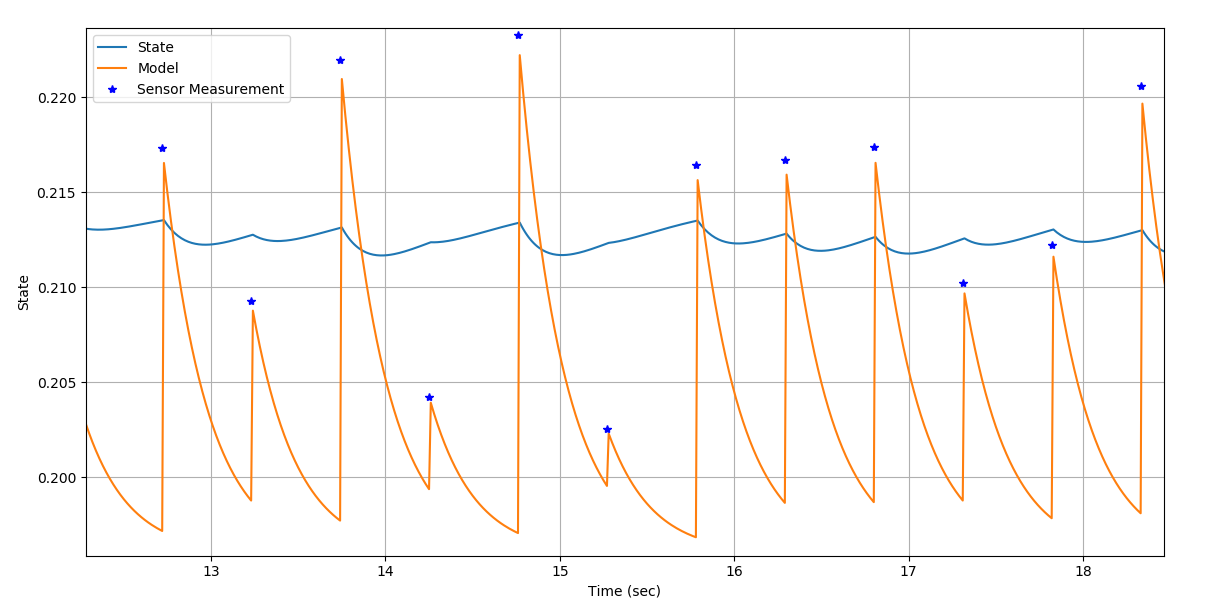
\includegraphics[height=80mm, width=140mm]{Figures/Kalman_Filter_Example.png}
  \end{center}
  \caption{First Order Kalman Filter Example}\label{f:kalman}
\end{figure}
    
\subsection{Kalman Filter for Spacecraft Dynamics}

Attitude estimation involves a combination of attitude determination
and state estimation. Assuming at time $t=t_0$ the attitude estimation
algorithm is performed and an estimate of the quaternion is obtained
as $\tilde{q}_0$. If discrete regular angular velocity
($\bar{\omega}_{k}$) measurements are made every $\Delta t$ seconds,
the quaternion can be estimated by simply integrating the attitude
equations of motion. Even if perfect sensor measurements are made, it
is possible to integrate these equations of motion over time and the
quaternion $\vec{q}$ will be much different than the estimated
quaternion $\tilde{q}$. Thus, the attitude estimation algorithm can
run again to obtain a new absolute quaternion measurement. The
equations of motion are integrated and when a new sensor measurement
is obtained the estimated state is updated based on the estimated
covariance combined with and estimate of model errors and sensor
errors. Finally, it is possible to 
create an Extended State Kalman Filter (EKF) which can estimate
sensor inaccuracies simply by finding the least squares solution
between the sensor measurements and state estimates. The sections that
follow details the Kalman Filter for Spacecraft Dynamics as well as
the extended state version which estimate bias values in the rate gyro.
  
First, the 4-dimensionality of the quaternion renders the
above Kalman filter formulation to be impossible mostly because the
quaternion derivative is a 4 by 1 matrix while the angular velocity
vector is a 3 by 1. Furthermore, the quaternion derivative is not
linear and cannot be expressed as the linear matrices in the previous
section. As such the Kalman Filter must be updated somewhat. The
derivative of the state $\dot{\vec{q}}$ is cumbersome and follows the
reference in \cite{Liu_Estimation}. First the angular 
velocity measurement is substituted into the derivative of
quaternions where the ${\bf \Omega}()$ and ${\bf \chi}()$ identity is used to
separate out the white noise parameter.
\begin{equation}
  \dot{\vec{q}} = \frac{1}{2}{\bf \Omega}(\vec{\omega})\vec{q} =
  \frac{1}{2}{\bf \Omega}(\bar{\omega}-\vec{b}-\vec{\eta}_g)\vec{q} =
  \frac{1}{2}{\bf \Omega}(\bar{\omega}-\vec{b})\vec{q} - \frac{1}{2}{\bf \chi}(\vec{q})\vec{\eta}_g
\end{equation}
At this point an error quaternion is created using the difference
between $\vec{q}$ and $\tilde{q}$. Recall that the error quaternion is
given by the equation below. The full equation is shown in
\ref{e:quat_difference}. 
\begin{equation}
  \delta \vec{q} = \vec{q}~\Earth~\tilde{q}^{-1}
\end{equation}
The derivative of this difference quaternion is beyond the scope of
this report but can be found in \cite{kalman_quat}.
\begin{equation}
  \dot{\delta \vec{q}} = \begin{Bmatrix} 0 \\ -{\bf
      S}(\tilde{\omega})\delta \vec{\epsilon} \end{Bmatrix} +
  \frac{1}{2}{\bf \Omega}(\delta \vec{\omega})\delta \vec{q}
\end{equation}
where $\delta \vec{\omega} = \vec{\omega} - \tilde{\omega}$ and
$\delta \vec{\epsilon} = \vec{\epsilon} - \tilde{\epsilon}$. Recall
that $\tilde{\omega} = \bar{\omega}-\tilde{b}$. The second term in the
equation above can be expanded using the equations in Section
\ref{s:measurements}. Note that $\delta \vec{\omega}$ simplifies to
$-\delta \vec{b} - \vec{\eta}_g$ and $\dot{\delta \vec{q}} = [\dot{\delta q_0},\dot{\delta
    \vec{\epsilon}}]^T$. 
\begin{equation}
  \dot{\delta \vec{q}} = \begin{Bmatrix} 0 \\ -{\bf
      S}(\tilde{\omega})\delta \vec{\epsilon} \end{Bmatrix} -
  \frac{1}{2}\begin{Bmatrix} -\delta \vec{\epsilon}^T\delta \vec{b}
    \\ \delta q_0 \delta \vec{b} + {\bf S}(\delta
    \vec{\epsilon})\delta \vec{b} \end{Bmatrix} -
  \frac{1}{2}\begin{Bmatrix} -\delta \vec{\epsilon} \vec{\eta}_g
    \\ \delta q_0 \vec{\eta}_g + {\bf S}(\delta
    \vec{\epsilon})\vec{\eta}_g \end{Bmatrix}
\end{equation}
In order to proceed further, small angle
approximations are made such that $|\delta \vec{q}|<<1$. The latter 3
variables in the quaternion are further approximated as $\delta
\vec{\rho} = \delta \vec{\epsilon}$. In order to fit in with the standard
Kalman filter, the state vector $\vec{x} = \vec{\rho}$ and thus the state
dynamics $\dot{\delta \vec{x}}$ can then be written as
\begin{equation}
  \dot{\delta \vec{x}} = \dot{\delta \vec{\rho}} = -{\bf
    S}(\tilde{\omega})\delta \vec{d} - \frac{1}{2}\delta \vec{b} -
  \frac{1}{2}\vec{\eta}_g
\end{equation}
In order to extract the attitude quaternion from the approximated
state the following equations are used.
\begin{equation}
  \begin{matrix}
    \delta \vec{\epsilon} = \frac{\delta \vec{\rho}}{\sqrt{1+\delta
        \vec{\rho}^T\delta \vec{\rho}}} & q_0 = \frac{1}{\sqrt{1+\delta
        \vec{\rho}^T\delta \vec{\rho}}}
  \end{matrix}
\end{equation}

\subsection{Extended State Kalman Filter}

As shown in the previous section, a Kalman filter can be used to
estimate the state. The standard Kalman filter however can be extended
to include the bias of the angular velocity measurement. Thus the
state vector is augmented to be $\vec{x} = [\vec{q},\vec{b}]^T$. Since
the derivative of the bias is the white noise vector, the difference
state vector after much simplification is shown below.
\begin{equation}
  \dot{\delta \vec{x}} = \begin{Bmatrix} \dot{\delta \vec{\rho}}
    \\ \delta \vec{b} \end{Bmatrix} =
  \begin{bmatrix} -{\bf S}(\tilde{\omega}) & -\frac{1}{2}{\bf I}_{3x3} \\
    {\bf 0}_{3x3} & {\bf 0}_{3x3} \end{bmatrix}
  \begin{Bmatrix} \delta \vec{\rho} \\\delta \vec{b} \end{Bmatrix} +
  \begin{Bmatrix} -\frac{1}{2}\vec{\eta}_g \\ \vec{\eta}_b \end{Bmatrix}
\end{equation}
In this formulation $\delta \vec{b} = \vec{b} - \tilde{b}$. The
derivative is then $\delta \dot{\vec{b}} = \vec{\eta}_b - 0$. It is
assumed that the derivative of the estimate is zero and thus is only
updated when sensor measurements are made. The states equation above can be
reduced to the state space form shown below. 
\begin{equation}
  \dot{\delta \vec{x}} = {\bf A}\delta \vec{x} + \vec{\eta}
\end{equation}

\subsection{Vehicle State Sensors}

Vehicle State estimation is a fundamental portion of GNC and
requires the vehicle to determine it's orientation with respect to an
inertial frame as well as its position from an inertial reference
point. Some sensors are specific to the vehicle application but here
this section will discuss a standard INS (Inertial Navigation System)
which consists of a GPS (Global Positioning System) and an IMU
(Inertial Measurement Unit).

\subsubsection{Inertial Measurement Unit}

An inertial measurement unit (IMU) is a combination of three
sensors. An accelerometer, rate gyro and magnetometer. A magnetometer
is a device that measures the local magnetic field in the body frame
$\hat{\beta}_{B} = [\hat{\beta}_x,\hat{\beta}_y,\hat{\beta}_z]^T$\cite{qp33}. Note that the $\hat{}$ implies a measurement rather than the truth signal. Measurements from sensors are prone to bias, drift, scale factor, misalignment, noise and other sources of error that must be accounted for.
\begin{figure}[H]
  \begin{center}
  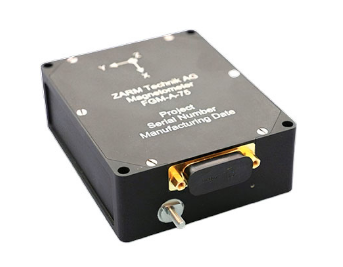
\includegraphics[height=50mm]{Figures/Magnetometer}
  \end{center}
  \caption{Example Magnetometer \cite{qp34}}
\end{figure}
A rate gyroscope, commonly referred to as a rate gyro measures the
angular velocity also in the body frame $\hat{\omega}_{B/I}=[\hat{g}_x,\hat{g}_y,\hat{g}_z]^T$. 
\begin{figure}[H]
  \begin{center}
  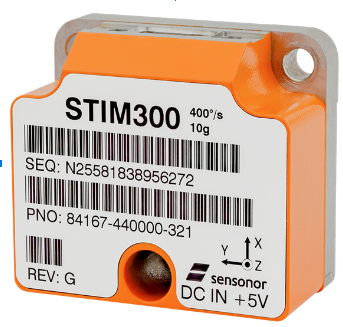
\includegraphics[height=50mm]{Figures/RateGyro}
  \end{center}
  \caption{Example IMU with Integrated Rate Gyro \cite{qp35}}
\end{figure}
Accelerometers are sensors used to measure acceleration at a point P
on a rigid body $\hat{a}_{B/I}=[\hat{a}_x,\hat{a}_y,\hat{a}_z]^T$. For simplicity however, it
is assumed that point P on the rigid body is the center of mass point
C therefore the accelerometer is measuring the acceleration of the
body itself in the body frame with respect to an inertial frame
$B/I$. 
\begin{figure}[H]
  \begin{center}
  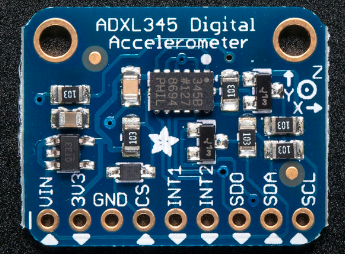
\includegraphics[height=50mm]{Figures/Accelerometer}
  \end{center}
  \caption{Example Accelerometer \cite{qp36}}
\end{figure}
As mentioned before, the IMU consists of 3 sensors all returning 3 measurments. This results in 9 scalar quantities being returned from this sensor which is where the term 9DOF gets it origin. In reality DOF means Degrees of Freedom which is contrary to the standard 6DOF simulation models explained above. However, the sensor community chooses to coin the term 9DOF to highlight the 9 different scalar values returned from IMUs. It is possible to obtain a 10DOF sensor which also returns pressure or temperature data. 

\subsubsection{Global Positioning System (GPS)}

The Global Positioning System (GPS) was developed in order to allow
accurate determination of geographical locations by military and civil
users. It works by using satellites in Earth’s orbit to transmit data
which makes it possible to measure the distance between the satellites
and the operator. This form of signal communication is incredibly
accurate and used heavily for attitude estimation. Up to 30 GPS
satellites are currently in orbit, mostly in MEO, at altitudes around
20,000 km. There will be between four and eight of them above any site
on the Earth at any time\cite{qp38}. These satellites continuously emit
coded high-frequency radio signals which may be received by special
GPS receivers. These signals contain information about the exact
orbits of the satellites and the time of atomic clocks onboard. When
signals from three or more satellites are received, the GPS receiver
will compute the best possible location of the user by
triangulation. Much like when on Earth, a GPS can be used for
navigation in space. The GPS receiver on board the satellite will also
receive its longitude, latitude, and altitude as long as it is within
the GPS constellation.
\begin{figure}[H]
  \begin{center}
  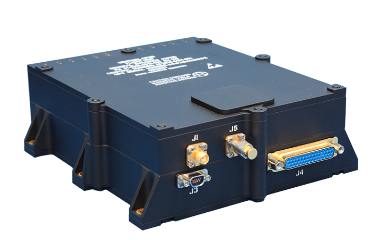
\includegraphics[height=50mm]{Figures/GPS}
  \end{center}
  \caption{Example GPS Receiver \cite{qp32}}
\end{figure}

\subsection{Euler Angle Estimation via IMU}

Using an IMU it is possible to obtain Euler Angles assuming a Flat Earth Approximation. Recall that Euler angles are a 3D transformation from the Inertial frame to the Body Frame (See Section \ref{s:Euler_Angles}). The angle $\phi$ and $\theta$ can directly be measured via the accelerometer by creating a relationship between the gravity vector in the inertial and body frames. The heading angle can be measured by creating a relationship between the magnetic field in the body frame and the inertial frame using a magnetometer. The rate gyro can be used to integrate the angular velocity to obtain Euler angles as well but is prone to drift. The accelerometer though is prone to errors when the vehicle experiences large acceleration loads. Thus, typically the Euler angles from the rate gyro are fused with the estimates from the magnetometer and the accelerometer. Still, some errors can still exist and the Euler angles can be fused with estimates from GPS but that will be explored in a separate section. First, let's examine the direct estimation of roll and pitch using the accelerometer. 

\subsubsection{Direct Measurement of Roll and Pitch}

Understand that the gravity vector in the inertial frame can be written as ${\bf C}_I(\vec{g}) = [0,0,g]^T$. However, since the first rotation in the Euler angle sequence is about the z-axis, the gravity vector in the A frame and Inertial (I) frames are identical. That is, ${\bf C}_A(\vec{g}) = {\bf C}_I(\vec{g})$. Normalizing the gravity vector yields ${\bf C}_A(\bar{g})=[0,0,1]^T$. The measurement from the accelerometer must also be normalized such that $\bar{a}_{B/I}=\hat{a}_{B/I}/||\hat{a}_{B/I}||$. Since the aircraft is always experiencing gravity, and the accelerometer is measuring the acceleration vector a relationship can be obtained between the gravity vector in the A frame and the acceleration vector in the body frame. Note that an assumption is being made here. It is assumed that the only acceleration being experienced is gravity. Therefore, if any external accelerations are experienced by the vehicle via thrust or aerodynamics, this equation is not valid. Still, for small UAV applications these equations can be accurate if fused properly with the rate gyro measurements. 
\begin{equation}
{\bf C}_B(\bar{a}_{B/I}) = {\bf T}_{NRB}^T{\bf T}_{ANR}^T{\bf C}_A(\bar{g}) = \begin{Bmatrix} -s_{\theta} \\ s_{\phi}c_{\theta} \\ c_{\phi}c_{\theta}\end{Bmatrix}
\end{equation}
The equation above takes the normalized gravity vector in the A frame and rotates it to the body frame through the no roll frame. Since the rotation is from the A frame to the body frame, only two rotations are required. Notice also that the first row can be used to obtain the pitch angle. 
\begin{equation}
\theta = -sin^{-1}(\bar{a}_x)
\end{equation}
The roll angle can then be obtained by taking the second two rows and dividing them together to get a tangent function. 
\begin{equation}
\phi = tan^{-1}\left(\frac{\bar{a}_y}{\bar{a}_z}\right)
\end{equation}
Note that this equation is only valid if $c_{\theta} \neq \pi/2$. This means the vehicle cannot fly straight up. For quadcopters and airplanes this is pretty typical for standard and level flight. For rockets however, either the IMU must be placed in an orientation that doesn't result in this singularity at launch or quaternions must be used. For spacecraft an entirely different algorithm is needed and is explained in a different section. 

Note that the pitch angle equation is written using the inverse sine function. Often times it is beneficial to compute the pitch angle using the inverse tangent function so that the {\it atan2} function may be utilized on a microcontroller which determines the quadrant of the angle more robustly. To do this the gravity vector must be written in the no roll frame. 
\begin{equation}
{\bf C}_{NR}(\bar{g}) = {\bf T}_{ANR}^T{\bf C}_A(\bar{g}) = \begin{Bmatrix} -s_{\theta} \\ 0 \\ c_{\theta}\end{Bmatrix}
\end{equation}
Then the acceleration vector is rotated to no roll frame as well from the body frame
\begin{equation}
{\bf C}_{NR}(\bar{a}_{B/I}) = {\bf T}_{NRB}{\bf C}_B(\bar{a}_{B/I}) = \begin{Bmatrix} \bar{a}_x \\ \bar{a}_y c_{\phi} - \bar{a}_z s_{\phi} \\ \bar{a}_y s_{\phi} + \bar{a}_z c_{\phi} \end{Bmatrix}
\end{equation}
Setting the two equations above equal to each other and diving the first row by the second row results in a tangent equation for pitch. This result is shown in the equation below.
\begin{equation}
\theta = -tan^{-1}\left(\frac{\bar{a}_x}{\bar{a}_y s_{\phi} + \bar{a}_z c_{\phi}}\right)
\end{equation}
Notice that these equations for pitch can be constructed by drawing a right triangle with the gravity vector as the hypotenuse. The sine function is the opposite side of the triangle divided by the hypotenuse which is 1 since the gravity vector was normalized while the inverse tangent function is the opposite side over the adjacent side. 

\subsubsection{Direct Measurement of Yaw}

In order to obtain the yaw angle of the vehicle through a direct measurement, the magnetometer is used. First it is assumed that the magnetic field strength is a constant through the flight of the vehicle and that it is oriented along the x-axis in the inertial frame of the Flat Earth Approximation. Remember that the x-axis is North using the Flat Earth Approximation. The magnetic field vector of the Earth is then normalized to unity. 
\begin{equation}
{\bf C}(\bar{\beta}_{\Earth}) = \begin{Bmatrix} 1 \\ 0 \\ 0 \end{Bmatrix}
\end{equation}
Again, in order to get a tangent function for the yaw angle estimation, the magnetic field of the Earth is written in the A frame. 
\begin{equation}
{\bf C}_A(\bar{\beta}_{\Earth}) = {\bf T}_{IA}^T{\bf C}_I(\bar{\beta}_{\Earth}) = \begin{Bmatrix} c_{\psi} \\ -s_{\psi} \\ 0 \end{Bmatrix}
\end{equation}
The magnetic field measurment of the magnetometer is then written in the A frame as well. However, the magnetometer measures the magnetic field in the body frame. Thus 2 rotations are requires to get from the body frame to the A frame. Again the magnetometer measurement is normalized.
\begin{equation}
{\bf C}_A(\bar{\beta}_{B}) = {\bf T}_{ANR}{\bf T}_{NRB}{\bf C}_B(\bar{\beta}_B)=\begin{Bmatrix} \bar{\beta}_x c_{\phi} + \bar{\beta}_y s_{\theta}s_{\phi} + \bar{\beta}_z c_{\phi}s_{\theta} \\ \bar{\beta}_y c_{\phi} - \bar{\beta}_z s_{\phi} \\ -\bar{\beta}_x s_{\theta} + \bar{\beta}_y s_{\phi}c_{\theta} + \bar{\beta}_z c_{\phi} c_{\theta} \end{Bmatrix}
\end{equation}
The two equations for magnetic field in the A frame can then be equated. In this case, the second row is divided by the first row to obtain a tangent relationship for yaw. The result for yaw is shown below.
\begin{equation}
\psi = tan^{-1}\left(\frac{\bar{\beta}_z s_{\phi} - \bar{\beta}_y c_{\phi}}{\bar{\beta}_x c_{\phi} + \bar{\beta}_y s_{\theta}s_{\phi} + \bar{\beta}_z c_{\phi}s_{\theta}}\right)
\end{equation}

\subsection{Low Earth Orbit Attitude Estimation}

In LEO the main algorithm begins with obtaining the magnetic field in
the body frame using magnetometers $\vec{\beta}_B$. Using the IGRF
model the locally measured magnetic field can be 
compared with the known magnetic field for any given location within
its orbit. Using the true data and the measured data, the spacecraft
can compute its actual position to the measured position and make the
correct adjustments. A Sun measurement is then taken using a Sun
sensor $\vec{S}_B$. Once those two independent 
body frame measurements are taken the inertial reference vectors must
be obtained from a database. Startrackers have this database built in;
however, for the magnetic field and the Sun vector these must be
obtained from a separate database as discussed in Section
\ref{s:ephemeris}. The idea is that if the position of the Earth is
known then the position of the Sun with respect to the Earth is also
known. The magnetic field vector can be 
obtained from the IGRF model as discussed in Section
\ref{s:magnetic_field}. The magnetic field vector in the inertial
frame is given as $\vec{\beta}_I$. Note that the IGRF model requires
the latitude and longitude to be known. Thus, in LEO a GPS is required
to feed into the database. The inertial Sun vector $\vec{S}_I$ only
requires the Julian time which can be obtained from GPS as well. The julian time is
based on the julian day as explained in Section \ref{s:ephemeris}.

The initial attitude determination algorithm itself requires two
independent vectors. As stated previously, startrackers provided a
large enough aperture and enough stars to produce the full
quaternion by obtaining multiple unique vectors to unique
stars. Multiple solar sensors or multiple magnetometers unfortunately
do not obtain non-unique vectors and the algorithm fails. In LEO this
is typically done with solar sensors and magnetometers but it can be
done with star trackers. In deep space it is typically done with
startrackers but it could be possible to obtain a Moon vector that
would require a Moon sensor.

The derivation below is done for the LEO case with a Sun and magnetic
field measurement. The derivation is identical for the deep space case
with a Moon sensor simply by substituting the magnetic field
measurment with a Moon measurement. Every vector is first normalized to obtain
$\hat{\beta}_B,\hat{\beta}_I,\hat{S}_B,\hat{S}_I$. A triad is then created
from body frame vectors using the equations below.
\begin{equation}
  \begin{matrix} \hat{f}_1 = \hat{S}_B & \hat{f}_2 = \hat{f}_1 \times
    \hat{\beta}_B & \hat{f}_3 = \hat{f}_1 \times \hat{f}_2 \end{matrix}
\end{equation}
The matrix ${\bf F}$ is then created using the triad as an orthonormal basis
$F = [\hat{f}_1,\hat{f}_2,\hat{f}_3]$. Similar equations are used for
the inertial measurements. 
\begin{equation}
  \begin{matrix} \hat{g}_1 = \hat{S}_I & \hat{g}_2 = \hat{g}_1 \times
    \hat{\beta}_I & \hat{g}_3 = \hat{g}_1 \times \hat{g}_2 \end{matrix}
\end{equation}
The matrix ${\bf G}$ is then created just as the ${\bf F}$ matrix such
that ${\bf G} =
[\hat{g}_1,\hat{g}_2,\hat{g}_3]$. The transformation from inertial to
body frame is then created using the formula below.
\begin{equation}
  {\bf T}_{BI} = {\bf FG}^T
\end{equation}
This matrix above is similar to the matrix in equation \ref{e:TIB} and
thus the Euler angles can be extracted from the matrix itself using
the formulation defined in Section \ref{s:Euler_Angles}. Euler can
then be converted to quaternions if needed. Note that it is relatively
easy to extract Euler angles from the ${\bf T}_{IB}$ matrix, it is not so
simple to extract quaternions. This is due to the fact that for every
orientation there exists two quaternions that represent this
space. Thus, it is more ideal to obtain Euler angles from the
transformation matrix and then convert them to quaternions.

\subsection{Spacecraft Position Estimation using a Ground Station Network (GSN)}

There are several types of ground stations depending on the
spacecraft’s distance from Earth. Ground services may be either
Direct-to-Earth (DTE) or space relay. DTE ground stations are located
on the Earth’s surface. They provide direct point-to-point access with
antennas at ground stations. DTE services are great for missions
needing frequent, short-duration contacts with high data transfer. 

Space relay services involve an intermediate satellite that
communicates with a ground station on the Earth’s surface. Relay
communication satellites for low-Earth orbit spacecraft can be in
Geosynchronous Equatorial Orbit (GEO), roughly 36,000 km from the
surface of Earth, or in low-Earth orbit. Relays are important for
providing communication and tracking when direct-to-ground
communications are not feasible due to physical asset visibility
constraints.  Space-based relay assets give missions full-time
coverage and continuous access to communication and tracking
services. 

Finally, deep space communication is also possible. The Deep Space
Network (DSN) is developed to conduct telecommunication and tracking
operations with space missions in GEO. This includes missions at lunar
distances, the Sun-Earth LaGrange points, and in highly elliptical
Earth orbits, and even missions to other planets\cite{qp40}. The DSN network
consists of three ground stations placed around 120 degrees apart on
Earth which provides 360 degrees coverage\cite{qp41}.
\begin{figure}[H]
  \begin{center}
  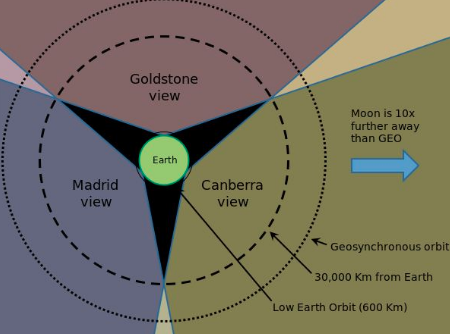
\includegraphics[height=80mm]{Figures/DSNSC}
  \end{center}
  \caption{Deep Space Network Satellite Coverage \cite{qp42}}
\end{figure}

\subsection{Heading Angle and Speed Estimation using GPS}

On Earth there is no need for a DSN because the vehicle is within the GPS constellation. Assuming the vehicle has the necessary GPS sensors a full NMEA (National Marine Electronics Association) can be obtained. However, in this example it is assumed that only the latitude, longitude and altitude coordinates are obtained in a discrete fashion. In order to get heading and speed it is assumed that consecutive measurements are obtained at $i$ and $i+1$ timestamps. Let's assume that the vehicle is traveling in a specific direction or heading and obtains a GPS coordinate $(\lambda_{LAT,i},\lambda_{LON,i},h_i)$ at time $t_i$. A few seconds later or whenever the update period may be the vehicle moves and the GPS returns a new GPS coordinate $(\lambda_{LAT,i+1},\lambda_{LON,i+1},h_{i+1})$ at time $t_{i+1}$. First, the coordinates are converted to a cartesian coordinate system. This is explained in the External Model section. This results in $x_i,y_i,z_i$ at time $t_i$ and $x_{i+1},y_{i+1},z_{i+1}$ at time $t_{i+1}$. First, the speed estimate is given by using a simple first order differentiation as given by
\begin{equation}
\begin{matrix}
v_x = (x_{i+1}-x_{i})/\Delta t \\
v_y = (y_{i+1}-y_{i})/\Delta t \\
\end{matrix}
\end{equation}
where $\Delta t = t_{i+1}-t_i$. Note that it is not recomended to compute the velocity in the z-axis as the altitude estimate of GPS is often not very good. Finally, the estimate for heading can follow from the speed estimate and is given as
\begin{equation}
\psi = tan^{-1}\left(\frac{v_y}{v_x}\right)
\end{equation}
Note that it is recommended to filter these estimates as GPS on its own is only accurate to around 3 meters.
